\documentclass{article} % For LaTeX2e
\usepackage{iclr2018_conference,times}
\usepackage{hyperref}
\usepackage{url}
\usepackage{graphicx}
\usepackage{epstopdf}
\usepackage{hyperref}
\usepackage{amsmath}
\usepackage{amsfonts}


\title{Numerical simulation on Black-Scholes model \\ Project Report}

% Authors must not appear in the submitted version. They should be hidden
% as long as the \iclrfinalcopy macro remains commented out below.
% Non-anonymous submissions will be rejected without review.

\author{Wenhao Yang\\
School of Mathematical Sciences\\
Peking University\\
\texttt{yangwenhaosms@pku.edu.cn} \\
}

% The \author macro works with any number of authors. There are two commands
% used to separate the names and addresses of multiple authors: \And and \AND.
%
% Using \And between authors leaves it to \LaTeX{} to determine where to break
% the lines. Using \AND forces a linebreak at that point. So, if \LaTeX{}
% puts 3 of 4 authors names on the first line, and the last on the second
% line, try using \AND instead of \And before the third author name.

\newcommand{\fix}{\marginpar{FIX}}
\newcommand{\new}{\marginpar{NEW}}
\iclrfinalcopy
%\iclrfinalcopy % Uncomment for camera-ready version, but NOT for submission.

\begin{document}
\graphicspath{{../result/}}
\maketitle

\begin{abstract}
In this report, I figure out the theoritical results and simulation results of stochastic differential equation on Black-Scholes model. The two simulation algorithms are Euler-Maruyama and Milstein scheme. Besides, multilevel monte carlo method is also applied to this model to make comparison with single monte carlo method.
\end{abstract}

\section{Model description and theoritical results}
In this section, I will give some theoritical results of Black-Scholes model. The stochastic differential equation of Black-Scholes model is:
\begin{align}
  dS_{t}=rS_{t}dt+\sigma S_{t}dW_{t}
\end{align}
And the exact solution of $S_{t}$ is: $S_{t}=S_{0}e^{(r-\frac{1}{2}\sigma^{2})t+\sigma W_{t}}$. In fact, we have:
\begin{align}
  d\log S_{t}&=\frac{1}{S_{t}}dS_{t}-\frac{1}{2S^{2}_{t}}(dS_{t})^{2}\notag\\
  &=rdt+\sigma dW_{t}-\frac{1}{2}\sigma^{2}dt\notag\\
  &=(r-\frac{1}{2}\sigma^{2})dt+\sigma dW_{t}\\
  \log S_{t}-\log S_{0}&=(r-\frac{1}{2}\sigma^{2})t+\sigma W_{t}\\
  S_{t}&=S_{0}e^{(r-\frac{1}{2}\sigma^{2})t+\sigma W_{t}}
\end{align}
And we care about the random variable $P=e^{-r}\max\{0,S_{1}-1\}$, which has following properties such as:
\begin{align}
  &\mathbb{P}(P=0)=\mathbb{P}(S_{1}\le 1)=\mathbb{P}(W_{1}\le\frac{1}{2}\sigma-\frac{r}{\sigma}-\frac{\log S_{0}}{\sigma})\\
  &\mathbb{P}(P>x)=\mathbb{P}(W_{1}>\frac{\log(xe^{r}+1)}{\sigma}-\frac{\log S_{0}}{\sigma}+\frac{\sigma}{2}-\frac{r}{\sigma})\\
  &\mathbb{E}[P]=\int_{0}^{+\infty}\mathbb{P}(P>x)dx
\end{align}
As it is difficult to get the exact value of the expectation of $P$, we just leave it alone. The next sections will compute its numerical simulation result.
\section{Numerical Approximation methods and Simulation results}
There are two mainly approximation methods to simulate the stochastic process.
\subsection{Euler-Maruyama Approximation}
The first approximation method is called Euler-Maruyama:
\begin{align}
  S_{t_{m+1}}^{(n)}=S_{t_{m}}^{(n)}+rS_{t_{m}}^{(n)}\Delta t_{m}+\sigma S_{t_{m}}^{(n)}\eta_{m}
\end{align}
where $\Delta t_{m}=T/n=\delta$ and $\eta_{m}=\Delta B_{t_{m}}\sim N(0,\delta)$

\subsection{Milstein Approximation}
The second approximation method is called Milstein:
\begin{align}
  S_{t_{m+1}}^{(n)}=S_{t_{m}}^{(n)}+rS_{t_{m}}^{(n)}\Delta t_{m}+\sigma S_{t_{m}}^{(n)}\eta_{m}+\frac{1}{2}\sigma^{2}S_{t_{m}}(\eta_{m}^{2}-\Delta t_{m})
\end{align}

\subsection{Simulation Results}
All of the parameters are set as: $S_{0}=1$, $r=0.05$ and $\sigma=0.2$. In order to compare the efficiency of the two simulation methods, mean absolute error is taken as quanlification. As the orders of these two simulation methods are not the same, $\sqrt{\delta}$ and $\delta$ are two orders for Euler-Maruyama and Milstein method, respectively.  The mean absolute errors of two simulation methods are shown in Fig~\ref{fig:1}, from which the Milstein method has a more quick convergence rate because of higher order.
\begin{figure}[htbp!]
  \centering
  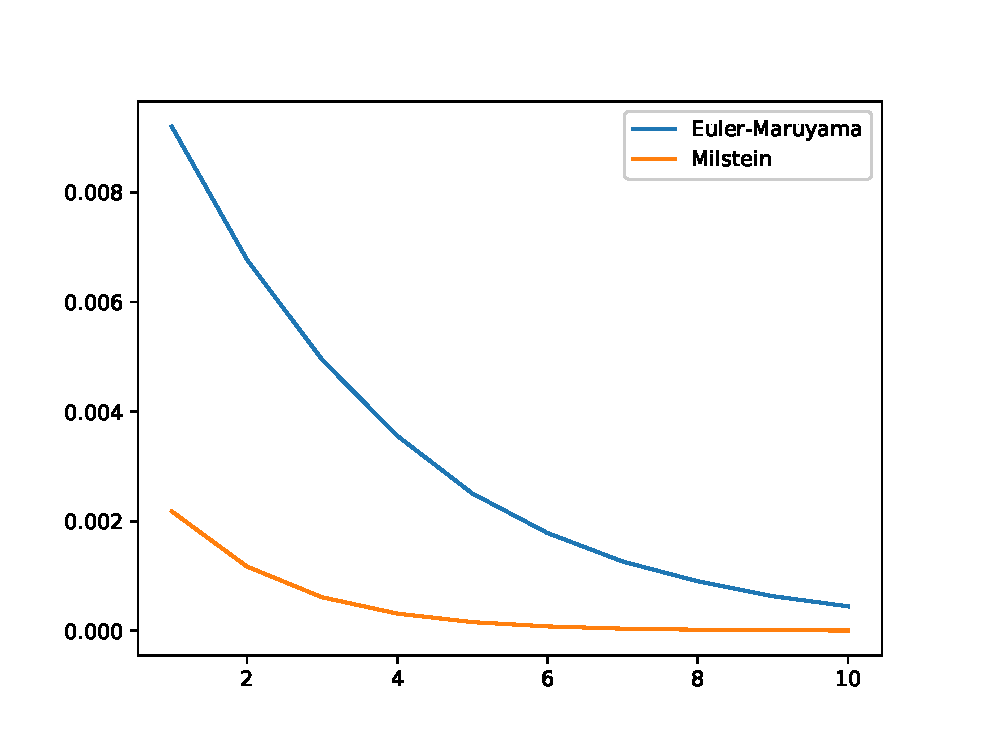
\includegraphics[width=\textwidth]{mc-strong.eps}
  \caption{Mean absolute errors}
  \label{fig:1}
\end{figure}

Besides of comparison of strong convergence, weak convergence is also plotted in Fig~\ref{fig:2}, from which the two methods have a nearly same convergence rate because they both have same order in terms of weak convergence.
\begin{figure}[htbp!]
  \centering
  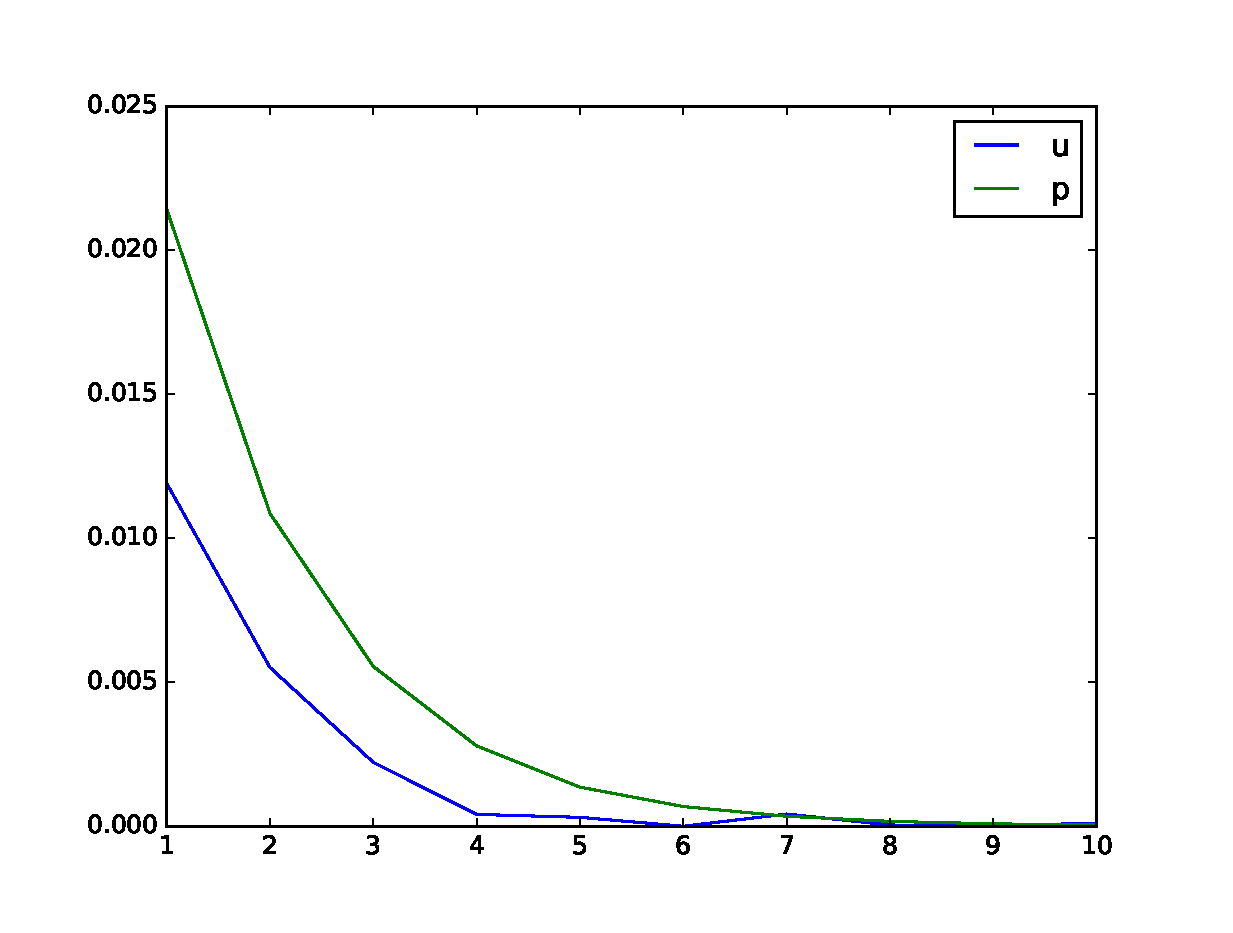
\includegraphics[width=\textwidth]{mc-weak.eps}
  \caption{Absolute mean errors}
  \label{fig:2}
\end{figure}


\section{Multilevel Monte Carlo Simulation method}

To reduce estimation variance, multilevel monte carlo is promoted. In this section, multilevel monte carlo method is used to simulate the Black-Scholes model.
\subsection{Multilevel Monte Carlo}
As our aim is to estimate the expectation $\mathbb{E}[f(S_{n, T})]$ to approximate $\mathbb{E}[f(S_{T})]$, where $n$ means discretize the time with $M^{-n}$. In this report, $M=2$ is always supposed. In fact the expectation can be rewritten as:
\begin{align}
  \mathbb{E}[f(S_{n, T})]=\mathbb{E}[f(S_{1, T})] + \sum_{k=2}^{n}\mathbb{E}[f(S_{k, T})-f(S_{k-1, T})]
\end{align}

So the estimation of $f(S_{n, T})$ could be written as:
\begin{align}
  \widehat{f}(S_{n, T})=\frac{1}{N_{1}}\sum_{i=1}^{N_{1}}f(S_{1, T}^{(i)})+\sum_{k=2}^{n}\frac{1}{N_{k}}\sum_{i=1}^{N_{k}}[f(S_{k, T}^{(i)})-f(S_{k-1, T}^{(i)})]
\end{align}

To reduce variance, for each $k$, $f(S_{k,T}^{(i)})-f(S_{k-1,T}^{(i)})$ is independent with $f(S_{k-1,T}^{(j)})-f(S_{k-2,T}^{(j)})$, which means, the estimation of $f(S_{k,T}^{(i)})-f(S_{k-1,T}^{(i)})$ is depended on the path simulated by $f(S_{k, T}^{(i)})$ instead of $f(S_{k-1, T}^{(j)})$. So the variance of $\widehat{f}(S_{n, T})$ is:
\begin{align}
  Var[\widehat{f}(S_{n, T})]=\sum_{k=1}^{n}\frac{V_{k}}{N_{k}}
\end{align}
where $V_{k}=Var[f(S_{k, T})-f(S_{k-1, T})]$
\subsection{Simulation Results}
All the parameters are set the same as before and the maximum level is set as $L=10$. For each level, $10^{6}$ times monte carlo is used to do estimation. Here we give an investigation on $V_{k}$ in Fig~\ref{fig:3}, where the x-axis is the level $l$ and y-axis is the estiamtion variance $V_{l}$. The variance reduces as level goes high. So we can simulate less for higher levels but higher for lower levels. Here we leave the variance of $V_{0}$ as it performs the same under both algorithms.
\begin{figure}[htbp!]
  \centering
  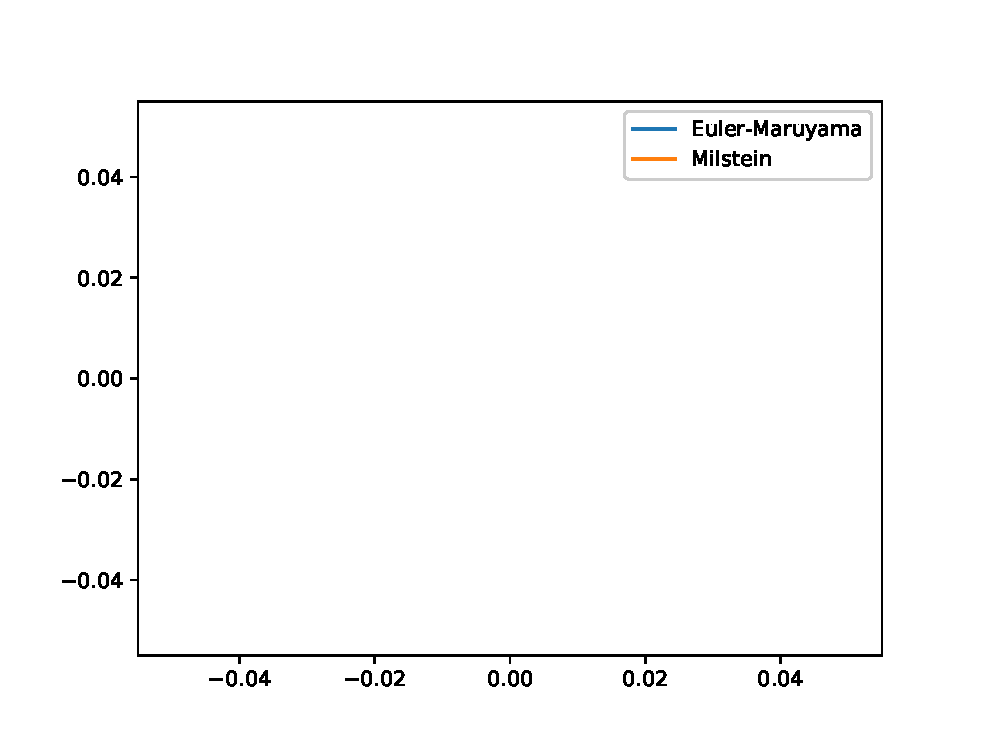
\includegraphics[width=\textwidth]{mmc-var.eps}
  \caption{Variance}
  \label{fig:3}
\end{figure}

According to \cite{Giles2008Multilevel}, the number of sampling at each level could be decided by:
\begin{align}
  N_{l} = \biggl\lceil 2\varepsilon^{-2}\sqrt{V_{l}h_{l}}(\sum_{l=0}^{L}\sqrt{V_{l}/h_{l}})\biggr\rceil\qquad
\end{align}
where $h_{l}=M^{-l}T$.

Different convergence accuracies $\varepsilon$ are set as $0.1,0.01,0.001,0.0001$. So the absolute mean errors $|\mathbb{E}f(S_{L, T}) - \mathbb{E}f(S_{T})|$ for different accuracy are shown in Fig~\ref{fig:4}, from which we could find that the two algorithms have nearly the same performace on convergence. That is because only weak convergence could be test while strong convergence can't compute because of multilevel estimation. So it is nothing strange to find out the same performance because these two algorithms have same weak convergence order.

However, it is not to say these two algorithms are the same good in terms of multilevel monte carlo. From Fig~\ref{fig:3} we find that Euler-Maruyama method has a higher variance than Milstein method, which means that Euler-Maruyama method should take more samples than Milstein method do. In terms of time cost, Milstein method has a better performance.
\begin{figure}[htbp!]
  \centering
  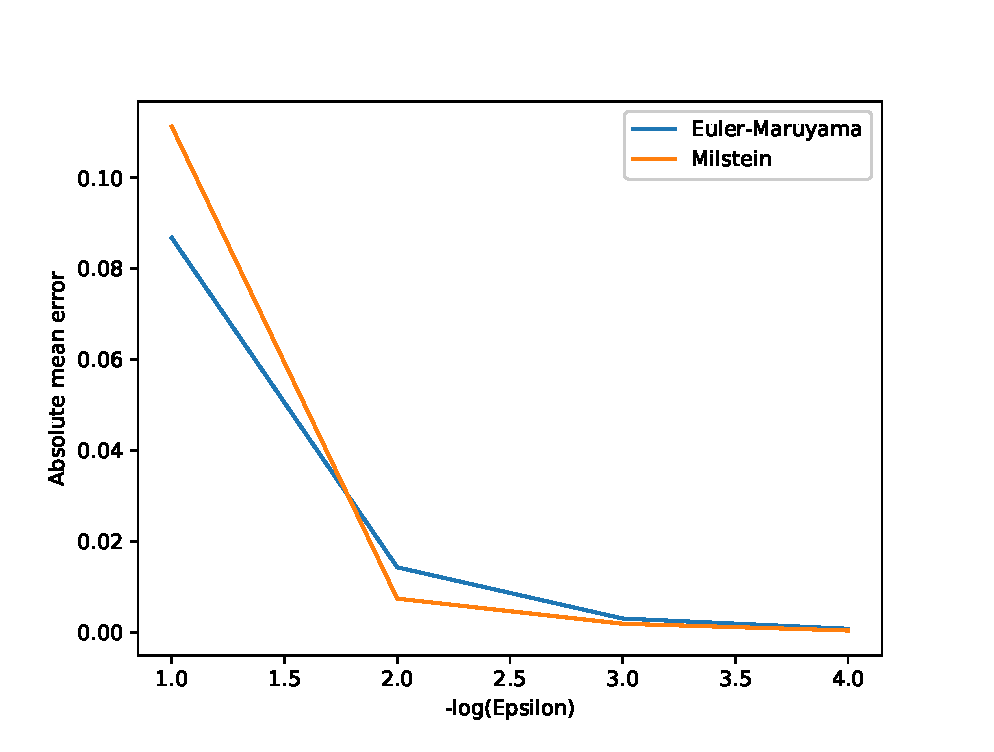
\includegraphics[width=\textwidth]{mmc-err.eps}
  \caption{Error}
  \label{fig:4}
\end{figure}

\subsubsection*{Experiment Details}
All of my code and results can be found on website \url{https://github.com/yangwenh/stochastic-simulation}. The mainly parallel method is asynchronized algorithm, which is implemented by ZMQ.

\subsubsection*{Acknowledgments}

I would like to thank Prof Li giving me a oppertunity to do research on stochastic differential equation. Thank Teaching Assistant Xiong helps to figure out my problems on the research topic. Thank Deep Learning Lab providing me computation resources.

\bibliography{iclr2018_conference}
\bibliographystyle{iclr2018_conference}

\end{document}
